\section{Results}\label{sec:result}
The measured $\sigma_{\mathrm{ABS}}$ and $\sigma_{\mathrm{CX}}$ are shown in Fig. \ref{fig:result} with statistical and systematic error bars as a function of pion momentum, compared with the results from previous experiments \cite{Bellotti1973,Ashery2,Bellotti1973_2,Jones}. Our results are in agreement with previous experiments, but we have extended the momentum region over which the data is presented. As summarized in Table \ref{table:systematics}, the total error is $\sim$9.5\% for $\sigma_{\mathrm{ABS}}$ and $\sim$18\% for $\sigma_{\mathrm{CX}}$, except for the $p_{\pi}$ = 216.6 MeV$/c$ data set.

\begin{figure}[h]
\begin{center}
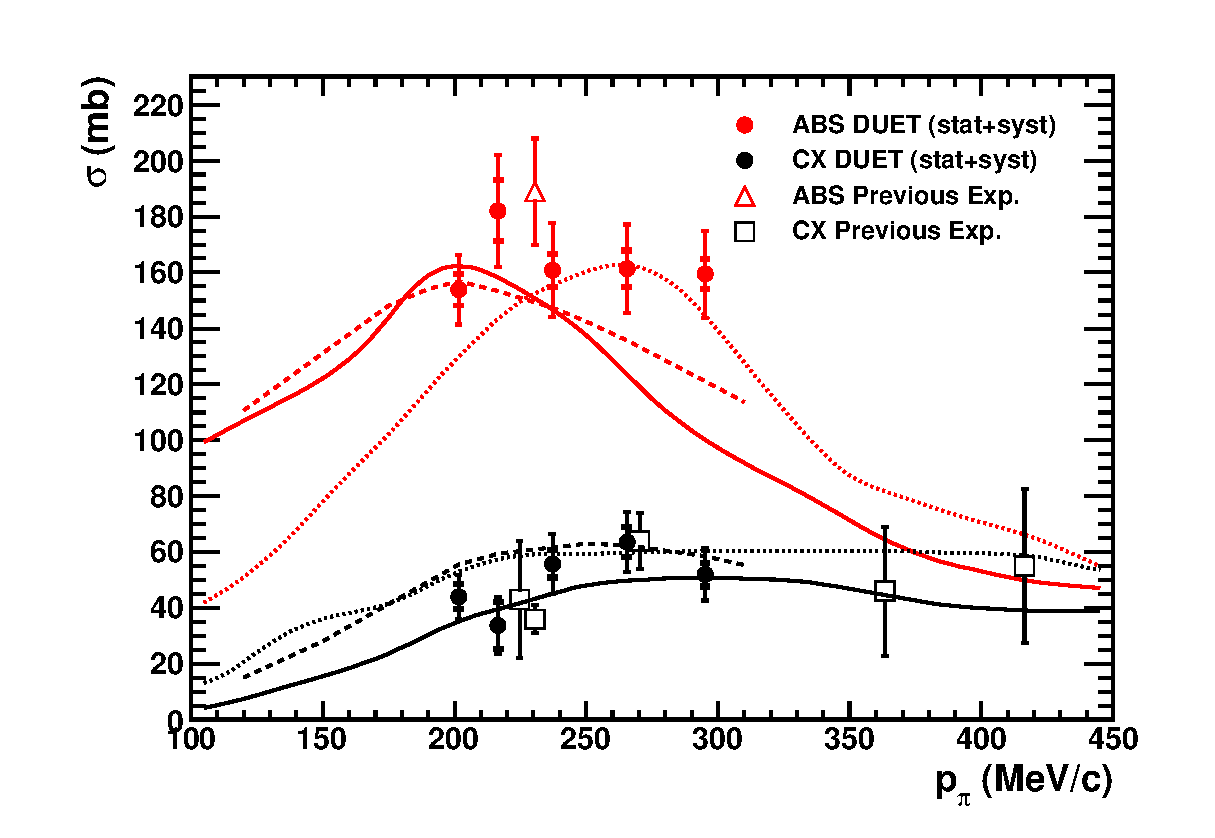
\includegraphics[width=86mm]{figures/duet_result_for_sep_paper.eps}
\caption{(Color online) DUET measurements of $\sigma_{\mathrm{ABS}}$ and $\sigma_{\mathrm{CX}}$ compared with previous measurements and ABS (red) and CX (black) model predictions from \textsc{Geant4} (solid line), \textsc{Fluka} (dashed line) and \textsc{Neut} (dotted line).}
\label{fig:result}
\end{center} 
\end{figure}

In addition, we provide the the fractional covariance matrix for the 5 $\sigma_{\mathrm{ABS}}$ and 5 $\sigma_{\mathrm{CX}}$ measured data points in Fig. \ref{fig:covariance}. The statistical uncertainties were included as an uncorrelated diagonal matrix. There are small positive correlations within the $\sigma_{\mathrm{ABS}}$ and 5 $\sigma_{\mathrm{CX}}$ measurements, and some negative correlations across them, as is expected from the subtraction method used. This is the first time that a correlation matrix is published for pion inelastic cross sections. It is expected to provide additional insight to the proper modeling and tuning of hadron-nucleus inelastic interactions.

\begin{figure}[h]
\begin{center}
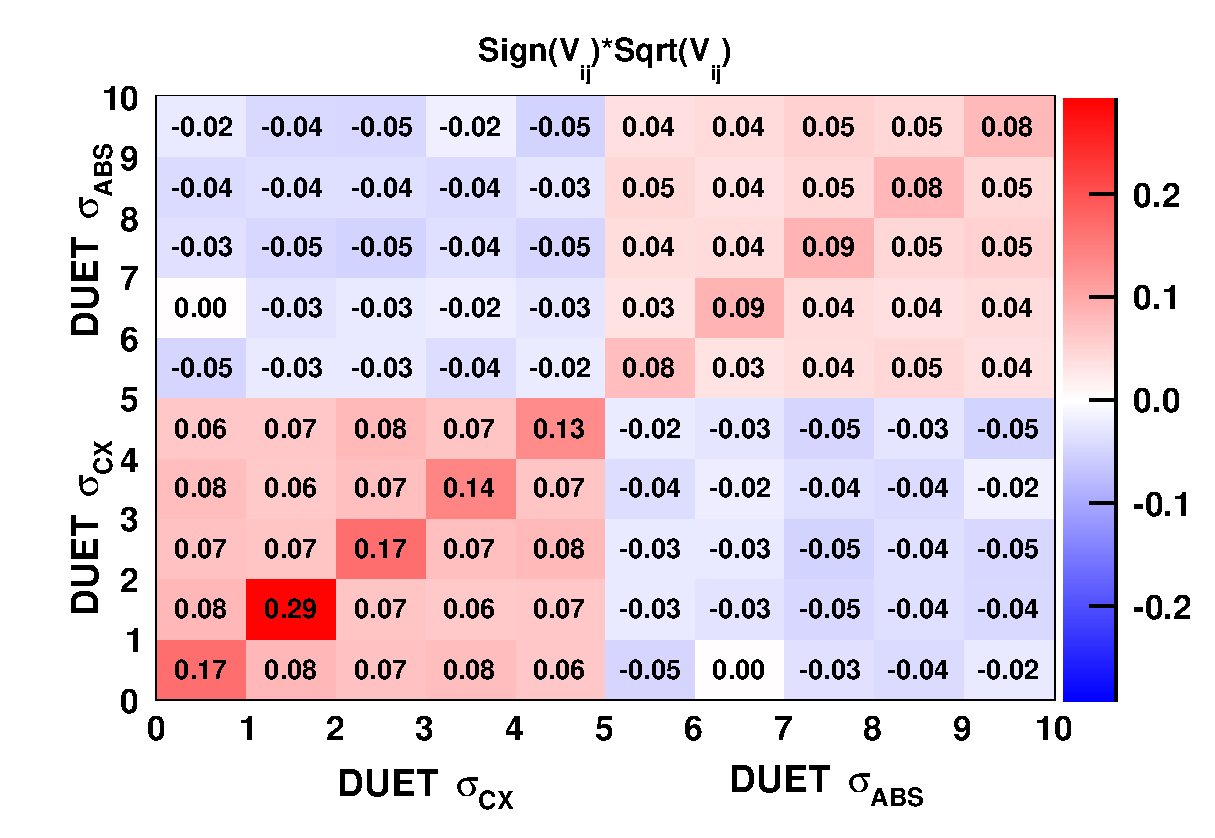
\includegraphics[width=86mm]{figures/duet_fractional_covariance_forpaper_v2.eps}
\caption{(Color online) Fractional covariance matrix for the DUET measurements of $\sigma_{\mathrm{ABS}}$ and $\sigma_{\mathrm{CX}}$. }
\label{fig:covariance}
\end{center} 
\end{figure}

\section{Summary}
To summarize, we obtained $\sigma_{\mathrm{ABS}}$ and $\sigma_{\mathrm{CX}}$ for positive pions in carbon nuclei at five incident momenta between 201.6 MeV$/c$ to 295.1 MeV$/c$. A covariance matrix for the 10 measured data points was produced. This result will be an important input to existing models such as \textsc{Geant4} or \textsc{NEUT} to constrain sub-GeV pion interactions.
